\begin{frame}[fragile]
 \frametitle{Liste annidate}
 \'E possibile creare liste di liste, di liste, di liste ...

 
\begin{block}{Esempio: Una lista annidata}
\begin{code}
\begin{minted}[linenos]{latex}
\begin{enumerate}
   \item Primo livello
   \begin{enumerate}
     \item Secondo livello
     \begin{enumerate}
       \item Terzo livello
     \end{enumerate}
   \end{enumerate}
 \end{enumerate}
\end{minted}
\end{code}
\end{block}
\end{frame}

\setbeamertemplate{enumerate items}[default]
\setbeamertemplate{enumerate item}{\arabic{enumi}}
\setbeamertemplate{enumerate subitem}{(\alph{enumii})}
\setbeamertemplate{enumerate subsubitem}{\roman{enumiii}}
%lavora schiavo

\begin{frame}[fragile]
 \frametitle{Liste annidate - 2}
 Il risultato è:
\begin{enumerate}
   \item Primo livello
   \begin{enumerate}
     \item Secondo livello
     \begin{enumerate}
       \item Terzo livello
     \end{enumerate}
   \end{enumerate}
 \end{enumerate}
\vspace{5mm}

\setbeamertemplate{enumerate items}[square]
\setbeamertemplate{enumerate item}{\arabic{enumi}}
\setbeamertemplate{enumerate subitem}{\arabic{enumi}.\arabic{enumii}}

La numerazione di default è:
\begin{enumerate}
    \item Numeri (1, 2, 3, ...) per il livello 1
    \item Lettere minuscole (a, b, c, ...) per il livello 2
    \item Numeri romani minuscoli (i, ii, iii, ...) per il livello 3
\end{enumerate}
\end{frame}
\begin{frame}[fragile]
 \frametitle{Liste annidate - 3}
Si può comunque modificare l'alfabeto del livello con il seguente comando
\begin{code}
\begin{minted}[linenos]{latex}
\renewcommand{\labelenumii}{\Roman{enumii}}
\end{minted}
\end{code}

\vspace{5mm}

\centering
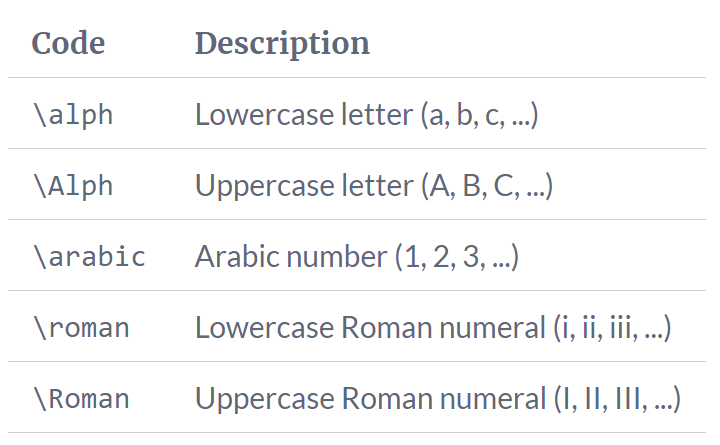
\includegraphics[scale=0.45]{ListeS}

\end{frame}

